%Knoten- und Maschenanalyse
\newpage

\newvideofile{KnotMasch}{Knoten- und Maschenanalyse}
\begin{frame}
	\fta{Knoten- und Maschenanalyse}

	\s{Bei der Betrachtung von elektrischen Netzwerken werden vor allem die Ströme 
    in Knoten und die Spannungen in Maschen analysiert. Die Analyse von Knoten und 
    Maschen in elektrischen Netzwerken erfolgt durch die beiden Kirchhoffsche Regeln.}

    \b{Die Analyse von Knoten und Maschen in elektrischen Netzwerken erfolgt durch 
    die Kirchhoffschen Regeln.}

    \begin{Lernziele}{Knoten- und Maschenanalyse}
        Die Studierenden 
        \begin{enumerate}
            \item kennen die grundlegenden Definitionen zur Beschreibung eines elektrischen Netzwerkes.
            \item können die Knotenregel und die Maschenregel auf elektrische Netzwerke anwenden. 
        \end{enumerate}
    \end{Lernziele}
    \speech{Knotmasch}{1}{
        Knoten und Maschen sind Definitionen, welche die Analyse von elektrischen Netzwerken 
        ermöglichen. Dabei werden die Knoten und Maschen eines elektrischen Netzwerkes mithilfe 
        der Kirchhoffschen Regeln behandelt. Hier soll erklärt werden, was die grundlegenden 
        Definitionen eines elektrischen Netzwerkes sind und wie die Knoten und Maschen mithilfe 
        der Kirchhofschen Regeln analysiert werden.}
\end{frame}




%Herleitung Knotenregel
\begin{frame}
    \ftb{Stromdichte im freien Raum} \label{Stromdichte}
 
    \s{
        Gegebenheiten und Begriffe aus der Feldtheorie führen zu den Erklärungen im
        strukturierten Feldraum. Dazu werden in der Abbildung \ref{BildStromdichte}
        eine positiv geladene Platte und eine negativ geladene Platte dargestellt,
        die sich gegenüberstehen. Der Raum zwischen den beiden Platten weist ein
        Elektrisches Feld $\vec{E}$ und ein Medium mit der Leitfähigkeit $\sigma$ auf. Ladungsträger
        können sich in dem freien Raum bewegen. Es stellt sich eine gerichtete Bewegung
        von Ladungsträgern und damit eine Stromdichte $\vec{J}$ zwischen den Platten ein.
        Die Stromdichte ist dabei in der betrachteten Fläche quellenfrei.
    }

    \b{Elektrisches Feld $\vec{E}$ zwischen zwei geladenen Platten:
    \begin{itemize}
        \item<1->   Raum zwischen den Platten ist mit einem leitfähigen Material $\sigma$ gefüllt
        \item<2->   Stromdichte $\vec{J}$ im elektrischen Feld 
        \item<3->   Quellenfreiheit der Stromdichte (Kontinuitätsgleichung)
    \end{itemize}}

    \fu{
        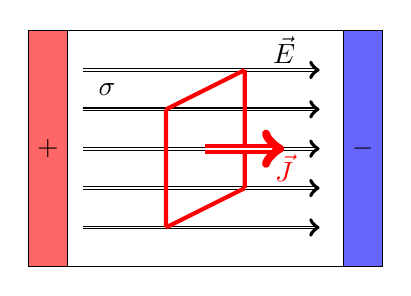
\begin{tikzpicture}
    \draw [fill=red!60] (0,0) rectangle (0.5,3) 
    (0.25,1.5) node {$+$};
    \draw (0.5,0) rectangle (4,3);
    \draw [fill=blue!60] (4,0) rectangle (4.5,3) 
    (4.25,1.5) node {$-$};
    \draw[double,->] (0.7,0.5) -- (3.7,0.5);
    \draw[double,->] (0.7,1) -- (3.7,1);
    \draw[double,->] (0.7,1.5) -- (3.7,1.5);
    \draw[double,->] (0.7,2) -- (3.7,2);
    \draw[double,->] (0.7,2.5) -- (3.7,2.5);
    \draw(1,2.25) node {$\sigma$};
    \draw(3.25,2.75) node {$\vec{E}$};
    \pause

    \draw[line width = 1.5, red] 
    (1.75,2) -- (2.75,2.5)
    (2.75,2.5) -- (2.75,1)
    (2.75,1) -- (1.75,0.5)
    (1.75,0.5) -- (1.75,2)
    (3.25,1.25) node {$\vec{J}$};
    \draw[double,->,line width = 1.5, red] (2.25,1.5) -- (3.25,1.5);
\end{tikzpicture}
        }{{\bf Elektrisches Feld zwischen einer positiv geladenen und einer negativ geladenen 
        Platte.} Die Stromdichte einer Beispielfläche im elektrischen Feld ist quellenfrei. 
        \label{BildStromdichte}}

    \s{
        Die Quellenfreiheit der Stromdichte wird durch die Gleichung \ref{divJQuellenfreiheit} 
        verdeutlicht. Hier wird beschrieben, dass keine Quellen oder Senken existieren, da sich 
        keine feldbildenden Ladungen im Raum befinden. Für diesen Fall ist die Stromdichte 
        quellenfrei und es fließen dieselbe Anzahl an Ladungen in die Fläche hinein und wieder heraus.
        Mathematisch wird dies für die Betrachtung im freien Raum in der Kontinuitätsgleichung ausgedrückt:
    }

    \only<3->{
    \begin{eq}
        \oint_{}^{} \vec{J} d\vec{A} = 0 \quad \rightarrow \quad div \vec{J} = 0 \label{divJQuellenfreiheit}
    \end{eq}
    }
    
    \speech{StromdichteimfreienRaum}{1}{
        Zuvor jedoch noch ein paar Grundlagen. Es wird ein elektrisches Feld E, zwischen einer positiv geladenen Platte, 
        hier in rot, und einer negativ geladenen Platte, hier in blau, betrachtet. Der Raum zwischen den beiden geladenen
        Platten ist mit einem leitfähigen Material Sigma, gefüllt und geometrisch nicht näher definiert.}
    \speech{StromdichteimfreienRaum}{2}{
        Aus dem elektrischen Feld E, resultiert eine theoretische Stromdichte J, im Raum zwischen den geladenen Platten.}
    \speech{StromdichteimfreienRaum}{3}{
        Die Kontinuitätsgleichung beschreibt das Oberflächenintegral der Stromdichte J, entlang einer geschlossenen Linie, 
        welche die Fläche A, einschließt, also dass die Stromdichte an jedem Punkt gleich ist und nicht zu- oder abnimmt. 
        Hiermit wird erklärt, dass die Divergenz der Stromdichte bei stetigen Strömen Quellenfrei beziehungsweise frei von 
        Senken ist.}
\end{frame}


\begin{frame}
	\ftb{Stromdichte im strukturierten Raum}

    \s{
        Im strukturierten Feldraum (vgl. Abbildung \ref{BildLeiterknoten}) gilt ebenfalls die Quellenfreiheit der Stromdichte. 
        Alle Ladungen, die in den Feldraum eindringen, müssen ihn auch wieder verlassen. 
        Dies gilt auch für den Fall, dass ein elektrischer Leiter mehr als einen Ableiter 
        aufweist. Es wird eine Zuleitung mit zwei Ableitungen 
        angedeutet, bei dem sich die Ladungen auf die beiden Ableitungen aufteilen. Die Zylinder-Mantelflächen
        $A_1$, $A_2$ und $A_3$ definieren mit den angrenzenden Zylindern einen strukturierten Feldraum. Wie die Ladungen teilen 
        sich die Stromdichten durch den strukturierten Raum auf. So ergibt sich die Stromdichte
        $\vec{J_1}$ aus der Summe der abfließenden Stromdichten $\vec{J_2}$ und $\vec{J_3}$. 
        
        \begin{columns}
        \column[c]{0.9\textwidth}  
        \fu{
            \begin{circuitikz}
    \draw
    [line width = 2.5, black]
    (0,0) circle (28pt)
    (0,1) -- (10,3)
    (0,-1) -- (5,0)
    (7,0.4) -- (10,1)
    (5,0) -- (5,-2.6)
    (7,0.4) -- (7,-2.6)
    (10,1) arc (-90:90:28.5pt)
    (5,-2.6) arc (-180:0:28.5pt);
    
    \draw[line width = 1.5, red][double,->] (1.5,0.3) -- (2.5,0.5);
    \draw[red](1.5,0.3) node[left] {$J_1$};
    \draw[line width = 1.5, red][double,->] (9,1.8) -- (10,2);
    \draw[red](10,2) node[right] {$J_2$};
    \draw[line width = 1.5, red][double,->] (6,-1.6) -- (6,-2.6);
    \draw[red](6,-2.6) node[below] {$J_3$};
 
    \draw
    [line width = 1.5, blue]
    (3,0.6) ellipse (22pt and 28pt)
    node at (3,0.6) {$A_1$}
    (8.5,1.7) ellipse (22pt and 28pt)
    node at (8.5,1.7) {$A_2$}
    (6,-1.1) ellipse (28pt and 22pt)
    node at (6,-1.1) {$A_3$};

    \draw[line width = 1.5, red][double,->] (5,1) -- (7,1.4);
    \draw[red](5,1) node[left] {$I_1$};
    \draw[red](7,1.4) node[right] {$I_2$};
    \draw[line width = 1.5, red][double,->] (6,1.2) -- (6,0.2);
    \draw[red](6,0.2) node[below] {$I_3$};

\end{circuitikz}
        }{{\bf Strukturierter Feldraum.} Vereinfachte Darstellung eines sich aufteilenden Leiters mit den Stromdichten 
        $J_1$, $J_2$ und $J_3$ und den Flächen $A_1$, $A_2$ und $A_3$.\label{BildLeiterknoten}}    
        \end{columns}

        Da der Feldraum im Beispiel durch die Flächen strukturiert und der Querschnitt der 
        Leitung definiert ist, lassen sich aus der Beziehung zwischen der Stromdichte und der 
        Fläche die Ströme der Leitungen gemäß Gleichung \ref{GleichungStromberechnung} ermitteln. 

        \begin{eq}
            I_1 = \iint_{A}^{} \vec{J_1} d\vec{A}  \label{GleichungStromberechnung}
        \end{eq}

        Der Zusammenhang der Stromdichten zueinander 
        lässt sich so auf die Ströme übertragen. Der Strom der Zuleitung $I_1$ ergibt sich aus der Summe der
        beiden Ableitungsströmen $I_2$ und $I_3$. Der Beispielleiter kann auch als vereinfachtes 
        elektrisches Netzwerk dargestellt werden. Die ermittelten Ströme um den Verbindungspunkt K (Knoten) 
        werden in der Abbildung \ref{BildKnotennetzwerk} abgebildet. 

        \fu{
            \begin{circuitikz}
    \draw
    (0,0) to [short, i=\red{$I_1$},-*] (2,0)
    (2,0) to [short, i=\red{$I_2$}] (4,0)
    (2,0) to [short, i=\red{$I_3$}] (2,-2);
    \draw[black](2,0) node[above] {$K$};

\end{circuitikz}
        }{{\bf Beispielknoten aus dem strukturierten Raum.} Aus den Stromdichten $J_1$, $J_2$ und $J_3$ ergeben sich um den Knoten K die Ströme 
        $I_1$, $I_2$ und $I_3$. \label{BildKnotennetzwerk}}
    }

    \b{
    
    Definierter Feldraum:

    \begin{minipage}[t]{0.7\textwidth}
        \begin{itemize}
            \item<2-> Bekannte Flächen und Stromdichten
            \item<3-> Strom
            \item<4-> Netzwerk
        \end{itemize}
    \end{minipage}
    \begin{minipage}[t]{0.29\textwidth}
        \only<3->{
        \begin{eq}
            I_1 = \iint_{A}^{} \vec{J_1} d\vec{A} 
        \end{eq}
        }
    \end{minipage}
    

    
    \begin{minipage}{1\textwidth}			
        \resizebox{\textwidth}{!}{\centering{
            \begin{circuitikz}
                \draw
                [line width = 2.5, black]
                (0,0) circle (28pt)
                (0,1) -- (10,3)
                (0,-1) -- (5,0)
                (7,0.4) -- (10,1)
                (5,0) -- (5,-2.6)
                (7,0.4) -- (7,-2.6)
                (10,1) arc (-90:90:28.5pt)
                (5,-2.6) arc (-180:0:28.5pt);
                \pause
                
                \draw[line width = 1.5, red][double,->] (1.5,0.3) -- (2.5,0.5);
                \draw[red](1.5,0.3) node[left] {$J_1$};
                \draw[line width = 1.5, red][double,->] (9,1.8) -- (10,2);
                \draw[red](10,2) node[right] {$J_2$};
                \draw[line width = 1.5, red][double,->] (6,-1.6) -- (6,-2.6);
                \draw[red](6,-2.6) node[below] {$J_3$};
                \draw
                [line width = 1.5, blue]
                (3,0.6) ellipse (14pt and 28pt)
                node at (3,0.6) {$A_1$}
                (8.5,1.7) ellipse (14pt and 28pt)
                node at (8.5,1.7) {$A_2$}
                (6,-1.1) ellipse (28pt and 14pt)
                node at (6,-1.1) {$A_3$};
                \pause

                \draw[line width = 1.5, red][double,->] (5,1) -- (7,1.4);
                \draw[red](5,1) node[left] {$I_1$};
                \draw[red](7,1.4) node[right] {$I_2$};
                \draw[line width = 1.5, red][double,->] (6,1.2) -- (6,0.2);
                \draw[red](6,0.2) node[below] {$I_3$};
                \pause

                \draw
                (15,0) to [short, i=\red{$I_1$},-*] (17,0)
                (17,0) to [short, i=\red{$I_2$}] (19,0)
                (17,0) to [short, i=\red{$I_3$}] (17,-2);
            \end{circuitikz}	
        }}	
    \end{minipage}
	} 
    
    \speech{StromdichteimstrukturiertenRaum}{1}{
        Zuvor haben wir die Stromdichte im freien Raum betrachtet. Jetzt soll die Stromdichte in einem strukturierten Raum,
        zum Beispiel in einem elektrischen Leiter, genauer Betrachtet werden.}
    \speech{StromdichteimstrukturiertenRaum}{2}{
        Im strukturierten Raum sind die Flächen des Raumes und die Stromdichten bekannt. Hier werden die Stromdichten J-Eins,
        J-Zwei und J-Drei mit ihren zugehörigen Flächen markiert.}
    \speech{StromdichteimstrukturiertenRaum}{3}{
        Aus den Stromdichten und den zugehörigen Flächen lassen sich die daraus resultierenden elektrischen Ströme bestimmen.
        Hier teilt sich der Strom I-Eins auf die Ströme I-Zwei und I-Drei auf.}
    \speech{StromdichteimstrukturiertenRaum}{4}{
        Die dreidimensionale Abzweigung im Leiter lässt sich auch als zweidimensionales elektrisches Netzwerk abbilden.}
\end{frame}

%Exkurs: Graphentheorie
\begin{frame}
    \ftb{Exkurs: Graphentheorie}
    
    \s{
        In der Mathematik beschäftigt sich die Graphentheorie mit der Beschreibung von
        Knoten und Kanten, in der Kontenanalyse werden ebenfalls Knoten und Äste definiert. 
        Durch die Graphentheorie können die Kanten und Knoten, welche in der Abbildung 
        \ref{GraphentheorieKnoten} dargestellt werden, sowie deren Eigenschaften 
        miteinander in Beziehung gesetzt werden. Über die Kanten können mehrere Knoten 
        miteinander verbunden werden.
    }

    \b{
        Beziehung zwischen Knoten und Ästen in der Graphentheorie:
        \begin{itemize}
            \item<2-> Kanten $\rightarrow$ Äste
            \item<3-> Knoten
        \end{itemize}
    }

    \begin{columns}
        
        \column[c]{0.3\textwidth}    
            \fu{
                \begin{circuitikz}
    \draw
    (0,0) to [short, -*] (2,0)
    (0,1.5) to [short] (2,0)
    (3.5,1.5) to [short] (2,0)
    (2,-2) to [short] (2,0);
    
    \pause
    \draw(2,1) node[above] {Kanten};

    \pause
    \draw[fill=red](2,0)circle(5pt);
    \draw[red](3,0) node[below] {Knoten};
\end{circuitikz}
            }{{\bf Beispielknoten der Graphentheorie.} Knoten mit 4 Kanten zur Erläuterung von Knoten und Kanten in der Graphentheorie.
            \label{GraphentheorieKnoten}}      
    \end{columns}
        
    \speech{KantenKnoten}{1}{
        Um elektrische Netzwerke einfacher beschreiben zu können, werden Bestandteile der Graphentheorie hinzugezogen.
        Die Graphentheorie wird in der Elektrotechnik zur Analyse von elektrischen Netzwerken und der Analyse von 
        Versorgungsnetzen eingesetzt.} 
    \speech{KantenKnoten}{2}{    
        Dafür werden Kanten, oder auch Äste definiert. Sie dienen als Verbindungswege zwischen zwei Punkten.}
    \speech{KantenKnoten}{3}{    
        Die Kanten können an Knoten zusammengeführt werden. Hier in rot markiert.}
\end{frame}

%Netzwerk und Matrix Graphentheorie
\begin{frame}
    \ftx{Exkurs: Graphentheorie}

    \s{
        Werden mehrere Knoten mit ihren Kanten miteinander verbunden entsteht ein Graph. Mit diesem 
        Graph kann exemplarisch ein elektrisches Netzwerk beschrieben werden. 
        Das Beispiel eines Netzwerkes mit fünf Knoten und den zwischen den Knoten liegenden Kanten
        wird in der Abbildung \ref{GraphentheorieNetzwerk} gezeigt. Wird ein Weg durch das Netzwerk
        gesucht ergeben sich unterschiedliche Möglichkeiten. Ein Weg vom Knoten 1 über die Knoten 2,
        4 und 5 zurück zum Knoten 1 wird rot hinterlegt. Sind Anfang und Ende derselbe Knoten, so wird 
        dieser Weg in der Graphentheorie auch als Zyklus bezeichnet. Jeder Zyklus, bei dem jeder Knoten 
        bis auf den Anfang und das Ende nur einmal „besucht“ wird, nennt man einen „Kreis“. In 
        elektrischen Netzwerken werden diese Kreise auch als Maschen bezeichnet. 
    }

    \b{
        Graph:
        \begin{itemize}
            \item<2-> Weg
            \item<3-> Weganfang = Wegende $\rightarrow$ Zyklus
            \item<4-> Kein kreuzender Zyklus $\rightarrow$ Kreis
        \end{itemize}
    }

   
    \fu{
        \begin{circuitikz}
    \draw
    (0,0) to [short, -*] (2,0)
    (0,0) node[above] {1}
    (2,0) to [short, -*] (4,0)
    (2,0) node[above] {2}
    (4,0) to [short, -*] (4,-2)
    (4,0) node[above] {3}
    (4,-2) to [short, -*] (2,-2)
    (4,-2) node[below] {4}
    (2,-2) to [short, -*] (0,0) 
    (2,0) to [short] (2,-2)
    (2,0) to [short] (4,-2)
    (2,-2) node[below] {5};

    \pause
    \draw [red, ->, very thick](0,0.05) to [short] (2,0.05);

    \pause
    \draw [red, ->, very thick](2.05,0) to [short] (4.05,-2);
    \draw [red, ->, very thick](4,-2.05) to [short] (2,-2.05);
    \draw [red, ->, very thick](1.95,-2) to [short] (-0.05,0);
\end{circuitikz}            
    }{{\bf Beispielnetzwerk der Graphentheorie.}
    Netzwerk mit 5 Knoten und zwischen den Knoten verlaufenden Kanten zur 
    Erläuterung eines Zyklus in der Graphentheorie. \label{GraphentheorieNetzwerk}}      


    \s{
        Um die Beziehung der Knoten untereinander zu erklären bietet sich in der Mathematik eine 
        Matrix an. Die Knoten weisen eine differenzierte Anzahl von Kanten auf und nicht alle Knoten sind 
        miteinander verbunden. Die Adjazenz-Matrix beschreibt die Beziehung der Knoten untereinander. 
        Eine solche Adjazenz-Matrix wird in der Gleichung \ref{AdjazenzMatrix} für das beschriebene
        Beispielnetzwerk aufgestellt. Sie beschreibt damit vollständig den Graphen, abgesehen von der grafischen 
        Repräsentanz in der 2D-Darstellung. 
    }

    \b{
        \onslide<5->{
            Zugehörige Adjazenz-Matrix:
        }
    }

    \onslide<5->{
    \begin{eq}
        A = 
        \begin{bmatrix}
            \color{blue}{1} & 1 & 0 & 0 & 1\\
            1 & \color{blue}{1} & 1 & 1 & 1\\
            0 & 1 & \color{blue}{1} & 1 & 0\\
            0 & 1 & 1 & \color{blue}{1} & 1\\
            1 & 1 & 0 & 1 & \color{blue}{1}
        \end{bmatrix} \label{AdjazenzMatrix}
    \end{eq}
    }

    \speech{Zyklus}{1}{
        Werden mehrere Kanten und Knoten verschaltet, ergibt sich daraus ein sogennanter Graf.} 
    \speech{Zyklus}{2}{    
        In diesem Graf lässt sich von einem beliebigen Knoten zu einem anderen Knoten ein Weg definieren.}
    \speech{Zyklus}{3}{    
        Ist der Knoten über andere Knoten hinweg sowohl Weg-Anfang als auch Weg-Ende ergibt sich daraus ein Zyklus.}
    \speech{Zyklus}{4}{    
        Wenn sich der Weg in einem Zyklus nicht kreuzt ergibt sich ein Kreis. Diese Kreise werden später bei der Analyse von 
        Maschen noch eine Rolle spielen.}
    \speech{Zyklus}{5}{    
        Die Beziehungen zwischen Knoten und Kanten in einem Graf können auch mathematisch durch die AdJazenz-Matrix beschrieben 
        werden. In die AdJazenz-Matrix wird eine Eins eingetragen, wenn ein Knoten über eine Kante einen direkten Weg zu einem 
        anderen Knoten hat. Für den Fall, dass keine direkte Verbindung zwischen zwei Knoten über eine Kante besteht, wird eine 
        Null notiert.}
\end{frame}

\begin{frame}
    \ftx{Graphentheorie}

    \begin{Merksatz}{Graphentheorie}
        In der Graphentheorie werden Netzwerke mit Kanten und Knoten beschrieben. Bei der Analyse der Netzwerke werden Wege und Zyklen
        definiert. Ein durchgehender Zyklus mit einem identischen Startpunkt und Endpunkt wird als Kreis bezeichnet. 
    \end{Merksatz}

    \speech{Graphentheorie}{1}{
        In der Graphentheorie werden Netzwerke mit Kanten und Knoten beschrieben. Bei der Analyse der Netzwerke werden Wege und Zyklen
        definiert. Ein durchgehender Zyklus mit einem identischen Startpunkt und Endpunkt wird als Kreis bezeichnet.} 
\end{frame}


\begin{frame} 
	\ftb{Knoten, Zweig, Masche}

	\s{
		Ein elektrisches Netzwerk besteht aus Knoten, Zweigen und Maschen. Ein Zweig verbindet genau zwei Knoten durch 
		ein oder mehrere Schaltungselemente miteinander. Durch alle Elemente eines Zweiges fließt der gleiche Strom. 
		In Abbildung \ref{Netz1} existieren drei Zweige. Ein Zweig mit den Komponenten $R_1$, $R_5$ und $U_\mathrm{q1}$, ein 
		Zweig mit dem Widerstand $R_4$ und ein Zweig mit den Komponenten $R_2$, $R_3$ und $U_\mathrm{q2}$.

		Ein Knoten ist ein Punkt, an dem mindestens drei Anschlüsse der Schaltungselemente zusammenlaufen. Der Strom 
		kann sich hier also aufteilen. Das elektrische Potential ist hierbei für alle verbundenen Anschlüsse identisch. 
		Im Schaltplan wird ein Knoten durch einen ausgefüllten Kreis gekennzeichnet. Sind jedoch zwei oder mehrere 
		dieser Kreise nur durch eine Leitung miteinander verbunden, handelt es sich um einen einzigen Knoten, da das 
		Potential auch hier gleich ist. Ein Knoten wird mit $K_n$ bezeichnet.

		Eine Masche ist ein geschlossener Weg, der aus mindestens zwei Zweigen besteht. In dem Netz in Abbildung 
		\ref{Netz1} können drei Maschen definiert werden:
			\begin{itemize}
				\item $M_1$ bestehend aus $R_1$, $R_4$, $R_5$ und $U_\mathrm{q1}$
				\item $M_2$ bestehend aus $R_2$, $R_3$, $R_4$ und $U_\mathrm{q2}$
				\item $M_3$ bestehend aus $R_1$, $R_2$, $R_3$, $U_\mathrm{q2}$, $R_5$ und $U_\mathrm{q1}$
			\end{itemize}
		Eine Masche wird mit $M_\mathrm{n}$ bezeichnet. Die Umlaufrichtung ist dabei von Bedeutung und wird mit einem Pfeil 
		gekennzeichnet.
	}

	\fu{	
        \begin{circuitikz}
    \draw(0,0) to[V, V<, name=Uq1] (0,3);			
    \draw (6,3) to[R=$R_3$] (6,0);
    \draw (6,0) to[V, name=Uq2] (3,0);
    \draw (3,0) to[R=$R_5$] (0,0);
    \varrmore{Uq1}{$U_{q1}$};
    \varrmore{Uq2}{$U_{q2}$};
    \only<1-3>{ \draw (3,0) to[R=$R_4$, *-*] (3,3);}
    \only<4>{ \draw (3,0) to[R=$R_4$,*-*, i<, v<, name=R4] (3,3);
    \iarrmore{R4}{$I_3$};
    \varrmore{R4}{$U_4$};}
    \only<1-3>{ \draw (0,3) to[R=$R_1$] (3,3);}
    \only<4>{ \draw (0,3) to[R=$R_1$, i, name=R1] (3,3);
    \iarrmore{R1}{$I_1$};}
    \only<1-3>{ \draw (3,3) to[R=$R_2$] (6,3);}
    \only<4>{ \draw (3,3) to[R=$R_2$, i<, name=R2] (6,3);
    \iarrmore{R2}{$I_2$};}

                
    \only<2-4>{\draw[red](3,3.3) node{$K_1$};	
    \draw[red](3,-0.3) node{$K_2$};	}						
    
    \only<3-4>{\def\StartAngle{30}
    \def\EndAngle{320}
    \def\Radius{0.85cm}			
    \draw[voltage, <-] ([shift=(\StartAngle : \Radius)]1.5,1.5)  arc[start angle=\StartAngle, end angle=\EndAngle, radius=\Radius];
    \draw[voltage, <-] ([shift=(\StartAngle : \Radius)]4.8,1.5)  arc[start angle=\StartAngle, end angle=\EndAngle, radius=\Radius];
    \draw[voltage] (2,0.5) -- (1,0.5) arc (270:180:0.5) -- (0.5,2) arc(180:90:0.5) -- (5.15,2.5) arc(90:0:0.5) -- (5.65,1) arc(0:-90:0.5);
    \draw[voltage,->] (5.15,0.5) -- (4,0.5);					
    \draw[voltage](1.5,1.5) node{$M_1$};	
    \draw[voltage](4.8,1.5) node{$M_2$};	
    \draw[voltage](0.5,0.5) node{$M_3$};}
\end{circuitikz}
	}{{\bf Gleichstromnetzwerk. }Netzwerk mit {\color{red}Knoten}, Zweigen und {\color{blue}Maschen}\label{Netz1}}

    \speech{Knoten,Zweige,Maschen}{1}{ Im folgenden werden die Definitionen von Knoten, Zweigen und Maschen in elektrischen Netzwerken 
        näher erläutert. Hierfür wird das dargestellte elektrische Netzwerk genutzt. Wie schon im Exkurs zur Graphentheorie ausgeführt, 
        sind Kanten oder Äste Verbindungswege zwischen zwei Punkten. Diese Kanten werden in der Elektrotechnik als Zweige bezeichnet. 
        Dieses elektrische Netzwerk setzt sich aus insgesamt drei Zweigen zusammen .} 
    \speech{Knoten,Zweige,Maschen}{2}{ Die Punkte, welche in dem gezeigten Netzwerk verbunden werden, sind die Knoten Ka 1 und Ka 2 .} 
    \speech{Knoten,Zweige,Maschen}{3}{ Eine Masche beschreibt einen geschlossenen Weg, der aus mindestens zwei Zweigen besteht. In dem 
        Netzwerk können so beispielsweise die Masche M 1 über die Komponenten R 1, R 4, R 5 und U Q 1 sowie die Masche M 2 über die 
        Komponenten R 2, R 3, U Q 2 und R 4 bestimmt werden. Außerdem können Maschen auch über zweige hinaus andere Zweige kreuzen. So 
        kann in diesem elektrischen Netzwerk die Masche M 3 über die Komponenten R 1, R 2, R 3, U Q 2, R 5 und U Q 1 definiert werden .} 
    \speech{Knoten,Zweige,Maschen}{4}{Bei den Maschen ist die Umlaufrichtung von Bedeutung und wird mit einem Pfeil gekennzeichnet. ebenso
        werden die richtungen von elektrischen Strömen gekennzeichnet. Hierzu später mehr bei der Knotenregel und der Maschenregel. } 
\end{frame}	

\begin{frame}
    \ftx{Knoten, Zweige und Maschen}

    \begin{Merksatz}{Knoten, Zweige und Maschen}
        Elektrische Netzwerke werden analog zur Graphentheorie durch Knoten, Zweige und Maschen beschrieben. 
    \end{Merksatz}

    \speech{MerkeKZM}{1}{Elektrische Netzwerke werden analog zur Graphentheorie durch Knoten, Zweige und Maschen beschrieben. } 
\end{frame}



\begin{frame} 
	\ftb{Der vollständige Baum}
	\s{
		Für die weitere Analyse des Netzwerkes ist es notwendig, die Netzwerkgleichungen zu ermitteln. Dieses lineare 
		Gleichungssystem ist aber immer überbestimmt, weshalb es nötig wird, die Anzahl der Gleichungen zu reduzieren. 
		Dabei ist es wichtig, die linear abhängigen Gleichungen zu identifizieren und zu eliminieren.
		
		Die Knoten, Zweige und Maschen eines Netzwerkes können in einem Graph dargestellt werden, der nur die 
		Verbindungen untereinander darstellt. Zur Darstellung des Graphen werden alle Zweige als Linien dargestellt, 
		welche die Knoten verbinden. Der Inhalt des Zweiges ist dafür irrelevant. In Abbildung \ref{AbbGraph} ist ein 
		beispielhaftes Netz mit dem sich ergebenden Graphen dargestellt.}

	\fu{
		\begin{minipage}{0.4\textwidth}
			\b{\resizebox{\textwidth}{!}{\centering{
				\begin{circuitikz}
					\draw (0,0) to[short] (0,1.5) 
						to[V,v<, name=U0, *-*] (0,4.5)
						to[short] (0,6)
						to[V, name=U1] (3,6)
						to[short] (3,4.5)
						to[R=$R_3$, *-*](3,1.5)
						to[R=$R_4$](0,1.5);
					\draw (0,4.5) to[R=$R_2$] (3,1.5);
					\draw (0,4.5) to[R=$R_1$] (3,4.5)
						to[short] (4,4.5)
						to[short] (4,0)
						to[short] (3,0)
						to[I, name=I2] (0,0);
					\varrmore{U0}{$U_{0}$};
					\varrmore{U1}{$U_{1}$};
					\iarrmore{I2}{$I_{2}$};
				\end{circuitikz}
			}}}		
			\s{
				\begin{circuitikz}
    \draw (0,0) to[short] (0,1.5) 
    to[V,v<, name=U0, *-*] (0,4.5)
    to[short] (0,6)
    to[V, name=U1] (3,6)
    to[short] (3,4.5)
    to[R=$R_3$, *-*](3,1.5)
    to[R=$R_4$](0,1.5);
    \draw (0,4.5) to[R=$R_2$] (3,1.5);
    \draw (0,4.5) to[R=$R_1$] (3,4.5)
    to[short] (4,4.5)
    to[short] (4,0)
    to[short] (3,0)
    to[I, name=I2] (0,0);
    \varrmore{U0}{$U_{0}$};
    \varrmore{U1}{$U_{1}$};
    \iarrmore{I2}{$I_{2}$};
\end{circuitikz}
			}
		\end{minipage}\hfill\pause
		\begin{minipage}{0.26\textwidth}
			\resizebox{\textwidth}{!}{
				\begin{circuitikz}
    \draw(0,0) to[short,*-*] (2,0);
    \draw(2,0) to[short,*-*] (2,2);
    \draw(2,2) to[short,*-] (1,3);			
    \draw(1,3) to[short,-*] (0,2);
    \draw(0,2) to[short,*-*](0,0);
    \draw(0,0) to[short] (2,2);
    \draw(2,2) to[short] (0,2);
    \draw(0,2) to[short] (2,0);						 
\end{circuitikz}
			}
		\end{minipage}	
	}{{\bf Gleichstromnetzwerk und Graph.} Erzeugung des Graphen aus einem zu berechnenden Netzwerk\label{AbbGraph}}

    \speech{VollstandigeBaum}{1}{Bei der Analyse von elektrischen Netzwerken kann der vollständige Baum genutzt werden.}
    \speech{VollstandigeBaum}{2}{Der vollständige Baum erklärt dabei ein elektrisches Netzwerk als ein gebilde aus Zweigen und Knoten.}
         
\end{frame}

\begin{frame} 
	\ftx{Der vollständige Baum}\label{vollstbaum}
	
	\s{
		In diesem Graph kann ein vollständiger Baum aufgezeichnet werden, der alle Knoten enthält, aber selbst keine 
		Masche bildet. Die Baumzweige verbinden also alle Knoten miteinander, bilden aber keine geschlossene Linie. 
		Die Baumzweige können Abzweigungen bilden, ein Knoten kann also auch mehr als zwei Baumzweige berühren.	In 
		größeren Netzwerken gibt es mehrere Möglichkeiten für einen vollständigen Baum, die prinzipiell gleichwertig 
		sind. Bei der Vorstellung der verschiedenen Berechnungsverfahren werden aber abhängig vom Verfahren 
		bestimmte Kombinationen bevorzugt. Ein vollständiger Baum beinhaltet genau $k-1$ Zweige.
		}
	
	\fu{
		\begin{minipage}{0.19\textwidth}
			\begin{circuitikz}
    \draw(0,0)[red, thick, densely dashed] to[short] (2,0);
    \draw(2,0)[red, thick, densely dashed] to[short] (2,2);
    \draw(2,2)[red, thick, densely dashed] to[short] (1,3);			
    \draw(1,3)[red, thick, densely dashed] to[short] (0,2);
    \draw(0,2) to[short,*-*](0,0);
    \draw(0,0) to[short, -*] (2,2);
    \draw(2,2) to[short, *-*] (0,2);
    \draw(0,2) to[short, -*] (2,0);						 
\end{circuitikz}
		\end{minipage}
		\hspace{0.2cm}
		\begin{minipage}{0.19\textwidth}
			\begin{circuitikz}
    \draw(0,0)[red, thick, densely dashed] to[short] (2,0);
    \draw(2,0)[red, thick, densely dashed] to[short] (2,2);
    \draw(2,2) to[short,*-] (1,3);			
    \draw(1,3) to[short,-*] (0,2);
    \draw(0,2)[red, thick, densely dashed] to[short](0,0);
    \draw(0,0) to[short, *-] (2,2);
    \draw(2,2) to[short] (0,2);
    \draw(0,2) to[short, -*] (2,0);						 
\end{circuitikz}
		\end{minipage}
		\hspace{0.2cm}
		\begin{minipage}{0.19\textwidth}
			\begin{circuitikz}
    \draw(0,0) to[short,*-*] (2,0);
    \draw(2,0) to[short,-*] (2,2);
    \draw(2,2) to[short] (1,3);			
    \draw(1,3) to[short,-*] (0,2);
    \draw(0,2) to[short](0,0);
    \draw(0,0)[red, thick, densely dashed] to[short] (2,2);
    \draw(2,2)[red, thick, densely dashed] to[short] (0,2);
    \draw(0,2)[red, thick, densely dashed] to[short] (2,0);						 
\end{circuitikz}
		\end{minipage}	
		\hspace{0.2cm}
		\begin{minipage}{0.19\textwidth}
			\begin{circuitikz}
    \draw(0,0)[red, thick, densely dashed] to[short, *-] (2,0);
    \draw(2,0) to[short,*-*] (2,2);
    \draw(2,2) to[short] (1,3);			
    \draw(1,3) to[short,-*] (0,2);
    \draw(0,2)[red, thick, densely dashed] to[short](0,0);
    \draw(0,0)[red, thick, densely dashed] to[short] (2,2);
    \draw(2,2) to[short] (0,2);
    \draw(0,2) to[short] (2,0);						 
\end{circuitikz}
		\end{minipage}
	}{{\bf Beispielbäume.} Beispiele für verschiedene in rot gezeichnete vollständige Bäume eines Netzes}
	
	\b{
		\begin{itemize}
			\item<2-> \red{Baumzweige} $\rightarrow$ k-1 des vollständigen Baumes
			\item<2-> die übrigen Zweige sind Verbindungszweige
		\end{itemize}
	}

	\s{
		Die Zweige, die zum Baum gehören, werden Baumzweige (rot), die anderen Verbindungszweige (schwarz) genannt.
		Um die linear unabhängigen Maschen zu finden, wird zu jedem Verbindungszweig eine Masche gebildet, die außer 
		dem Verbindungszweig nur Baumzweige enthält.
		}
    \begin{itemize}
        \item<3-> Ein Netzwerk mit $z$ Zweigen und $k$ Knoten enthält $z-k+1$ Verbindungszweige.
    \end{itemize}
	
    \speech{VollstandigeBaumBsp}{1}{Beim vollständigen Baum gibt es eine vielzahl an möglichen Anordnungen von verwendeten Zweigen.}
    \speech{VollstandigeBaumBsp}{2}{Hierbei muss zwischen den hier in rot gestrichelten Baumzweigen und den Verbindungszweigen 
    unterschieden werden. Es gibt in einem elektrischen Netzwerk immer k minus eins Baumzweige. Über die Baumzweige werden alle Knoten
    miteinander verbunden, ohne dabei eine Masche zu definieren, also ohne, dass ein Knoten zwei mal berührt wird. 
    Die übrigen Zweige werden als Verbindungszweige definiert. }
    \speech{VollstandigeBaumBsp}{3}{Ein Netzwerk mit Z Zweigen und K Knoten enthält Z minus K plus eins Verbindungszweige.
    Die Anzahl der Verbindungszweige entspricht später auch der Anzahl der unabhängigen Maschengleichungen, welche nötig sind, 
    um ein elektrisches Netzwerk zu analysieren.}

\end{frame}

\begin{frame}
    \ftx{Der vollständige Baum}

    \begin{Merksatz}{Der vollständige Baum}
        Mithilfe eines vollständigen Baumes werden alle Knoten miteinander durch Baumzweige verbunden. 
        Es ergeben sich dabei immer k - 1 Baumzweige. 
        Der vollständige Baum bildet keine Masche. 
    \end{Merksatz}

    \speech{VollstandigeBaumMrk}{1}{Mithilfe eines vollständigen Baumes werden alle Knoten miteinander durch Baumzweige verbunden.
    Es ergeben sich dabei immer k minus 1 Baumzweige. Der vollständige Baum bildet keine Masche.}
\end{frame}


%Knotenregel
%Knotenregel Summenzeichnen
\begin{frame}
    \ftb{Knotenregel}

    \s{
        Treffen sich mehr als zwei Leitungen an einem Punkt eines elektrischen 
        Netzwerkes handelt es sich um einen Knotenpunkt K. Die Pfeilrichtung aus 
        der Sicht des Knotens bestimmt das Vorzeichen des Stromes. Führt ein Strom 
        in einen Knoten hinein, so zeigt der Strompfeil auf den Knoten und es handelt 
        sich um eine Einströmung. Zeigt der Strompfeil aus dem Knoten heraus, wird 
        der Strom aus dem Knoten herausgeführt und es handelt sich um eine Ausströmung. 
        Die Knotenanalyse ergibt sich aus dem 1. Kirschhoff`schen Gesetz, welches besagt: 
        Die Summe aller Ströme an einem Knoten ist Null (Gleichung \ref{Knotenregel}). 
        Dieses Gesetz folgt direkt aus der Kontinuitätsgleichung (vgl. Abschnitt 
        \nameref{Stromdichte})
    }

    \b{ 
        \begin{itemize}
            \item Die Summe aller Ströme an einem Knoten ist gleich Null.
        \end{itemize}
    }

    \begin{eq}
        \sum_{k = 1}^{N}{I_\mathrm{k} = 0} \label{Knotenregel}
    \end{eq}
    
    \s{
        So müssen sich für jeden Knoten die Summe der Stromstärken aus Einströmungen 
        und Ausströmungen gegenseitig ausgleichen. In der Abbildung \ref{BildBeispielknoten} sind ein 
        Knoten K und die Ein- und Ausströmungen eingezeichnet. Bei den Strömen $I_1$ und 
        $I_2$ handelt es sich um Einströmungen. Die drei Ströme $I_3$, $I_4$ und $I_5$ sind 
        Ausströmungen. 
    }

    \b{
        \begin{itemize}
            \item Beispielnetzwerk:
        \end{itemize}
    }

        \fu{
            \begin{circuitikz}
    \draw
    (0,1) to [short, i=\red{$I_1$},-*] (2,0)
    (0,-1) to [short, i=\red{$I_2$}] (2,0)
    (2,0) to [short, i=\red{$I_3$}] (3.5,1.5)
    (2,0) to [short, i=\red{$I_4$}] (4,0)
    (2,0) to [short, i=\red{$I_5$}] (3.5,-1.5);
\end{circuitikz}
        }{{\bf Beispielknoten.} Knoten für die Knotenanalyse mit zwei einströmenden und 
        drei ausströmenden Zweigen. \label{BildBeispielknoten}}


	\s{
		Werden die Ströme nacheinander aufgetragen und gleich Null gesetzt, ergibt 
		sich die Gleichung \ref{KnotenregelBeispielknoten}. Je nachdem ob es sich 
		um eine Einströmung oder eine Ausströmung handelt, wird das Vorzeichen 
		gewählt. Einströmungen werden mit einem positiven und Ausströmungen mit 
		einem negativen Vorzeichen behaftet. 
	}
    
    \b{
        \begin{itemize}
            \item Summe aus Einströmungen und Ausströmungen gleich null:
        \end{itemize}
    }
    
    \begin{eq}
        \sum_{k = 1}^{N}{I_\mathrm{k}} =0=I_1+I_2-I_3-I_4-I_5    \label{KnotenregelBeispielknoten}
    \end{eq}

    \speech{Knotenregel}{1}{Die Knotenregel beschreibt die Verhältnisse von elektrischen Strömen an einem Knoten und besagt, 
    dass die Summe aller Ströme an einem Knoten gleich null ist.
    Anhand des Beispielnetzwerkes mit den fünf Strömen soll die Knotenregel veranschaulicht werden. Bei den Strömen I 1 und I 2 handelt 
    es sich um elektrische Ströme die auf den Knoten zuströmen. Die Ströme I 3, I 4 und I 5 strömen von dem Knoten weg. 
    Sie Summe aus Einströmungen und Ausströmungen muss also gleich null sein.}
\end{frame}

\begin{frame}
    \ftx{Knotenregel}

    \begin{Merksatz}{Knotenregel}
        Die Summe der zufließenden Ströme ist gleich der Summe der abfließenden Ströme oder die Summe aller Ströme an einem Knoten
        ist Null:
        \begin{eq}
            \sum_{k = 1}^{N}{I_\mathrm{k} = 0} 
        \end{eq}
    \end{Merksatz}

    \speech{KnotenregelMrk}{1}{Die Summe der zufließenden Ströme ist gleich der Summe der abfließenden Ströme oder die Summe aller Ströme 
    an einem Knoten ist Null.}
\end{frame}



%Maschenanalyse
\begin{frame}
    \ftb{Maschenregel}

    \s{
		Bewegt sich ein Teilchen zwischen zwei Punkten in einem elektrischen Feld, wird Arbeit verrichtet. 
		Ist der Startpunkt identisch mit dem Endpunkt, muss ebenso viel Arbeit abgegeben wie aufgenommen werden. 
		Die Summe der Arbeit ist in diesem Fall gleich Null. Wenn so ein kompletter Maschenumlauf entlang einer 
		geschlossenen Strecke vollzogen wird, muss die Summe der Teilspannungen ebenfalls gleich Null sein. 
		Vorausgesetzt wird hier, dass sich keine zeitlich veränderte magnetische Flussdichte ergibt und somit kein 
		elektrisches Wirbelfeld entsteht (vgl. Gleichung \ref{GleichungRingintegralFeldstärke}). Die Gleichung
        beschreibt hier das Faradaysche Induktionsgesetz für statische Felder (hier: keine Änderung eines Magnetfeldes).
    }

    \b{
        Ringintegral über der Feldstärke: 
        \begin{itemize}
            \item Bedingung: Keine zeitlich veränderte magnetische flussdichte und somit kein elektrisches Wirbelfeld. 
        \end{itemize}
    }

    \begin{eq}
        \oint_{s}^{} \vec{E} d\vec{s} = 0 \quad \rightarrow \quad rot \vec{E} = 0 \label{GleichungRingintegralFeldstärke}
    \end{eq}

    \s{
        Die Maschenanalyse besagt nach der 2. Kirchhoffschen Regel, dass bei einem 
        vollständigen Umlauf (Masche) in einem elektrischen Netzwerk die Summe aller 
        Spannungen gleich Null ist. Dies wird durch die Gleichung \ref{Maschenregel} 
        verdeutlicht. 
    }

    \b{\onslide<2->{
        Maschenregel:
        \begin{itemize}
            \item Bei einem vollständigen Umlauf in einem elektrischen Netzwerk ist die Summe aller Spannungen gleich null. 
        \end{itemize}}
    }

    \onslide<2->{
    \begin{eq}
        \sum_{k = 1}^{N}{U_\mathrm{k}} =0    \label{Maschenregel}
    \end{eq}}

    \speech{Maschenregel}{1}{Tritt keine zeitliche Änderung bei elektrischen und magnetischen Feldgrößen auf, können keine 
    elektrischen Wirbelströme induziert werden. Bewegt sich unter dieser Bedingung ein Teilchen zwischen zwei Punkten im 
    elektrischen Feld, wird Arbeit verrichtet. Ist der Startpunkt identisch mit dem Endpunkt, muss ebenso viel Arbeit 
    abgegeben wie aufgenommen werden. Die Summe der Arbeit ist in diesem Fall gleich Null. Ähnlich zum Umlauf im freien Raum,
    wie dem elektrischen Feld, verhält sich ein Umlauf im strukturierten Raum, also in einem elektrischen Netzwerk.}
    \speech{Maschenregel}{2}{Hierzu wird die Maschenregel definiert. Die Maschenregel besagt, dass die Summe aller Teilspannungen 
    bei einem vollständigen Umlauf gleich null sein muss.}
\end{frame}

\begin{frame}
    \ftx{Maschenregel}
    
    \s{
        Innerhalb einer Masche werden die Spannungen mit einer gleichgerichteten Pfeilrichtung 
        positiv gezählt, Spannungen mit der Umlaufrichtung entgegengesetzten Pfeilrichtung werden 
        negativ gezählt. Ausgehend von den Stromverläufen und Potentialen aus der Abbildung
        \ref{BeispielnetzwerkMaschenanalyse} können die Spannungen der jeweiligen Zweige ermittelt 
        werden. Oberhalb der Parallelschaltung der Widerstände gibt es keine Potentialdifferenz. 
        Selbiges gilt für die elektrische Verbindung unterhalb der Parallelschaltung. Der Strom $I_\mathrm{R1}$ 
        fließt durch den Widerstand $R_\mathrm{1}$. So ergibt sich nach dem ohmschen Gesetz die Spannung $U_\mathrm{R1}$ 
        über $R_\mathrm{1}$. Äquivalent wird die Spannung $U_\mathrm{R2}$ über $R_\mathrm{2}$ bestimmt.
    }

	\fu{
		\begin{circuitikz}
    \draw (0,0) to [I, name=I0] (0,4)
    to [short,-*] (4,4)
    to [short] (8,4)
    (4,4) to [R=$R_\mathrm{1}$, v, i, name=R1] (4,0)
    (8,4) to [R=$R_\mathrm{2}$, v, i, name=R2] (8,0)
    to[short,-*] (4,0)
    to[short] (0,0);
    \draw[->,shift={(6,2)},voltage] (150:0.8) arc (150:-150:0.8) node at(0,0){$M_\mathrm{1}$};
    \varrmore{R1}{$U_\mathrm{R1}$};
    \iarrmore{R1}{$I_\mathrm{R1}$};
    \varrmore{R2}{$U_\mathrm{R2}$};
    \iarrmore{R2}{$I_\mathrm{R2}$};
    \iarrmore{I0}{$I_\mathrm{0}$};

\end{circuitikz}
	}{{\bf Beispielnetzwerk mit einer Stromquelle und zwei parallelen Widerständen.} In der Masche $M_1$ müssen die Spannungen
	$U_\mathrm{R1}$ und $U_\mathrm{R2}$ identisch sein und sich ensprechend ihrer Richtungen in der Masche aufheben. \label{BeispielnetzwerkMaschenanalyse}}

    \s{
        Gemäß des vorgestellten Netzwerkes und der Richtung der eingezeichneten Masche $M_\mathrm{1}$ stellt
        sich der Zusammenhang nach Gleichung \ref{Maschengleichung} ein. Die Spannung $U_\mathrm{R2}$ verläuft 
        in derselben Richtung, wie die eingezeichnete Masche und wird mit einem positiven Vorzeichen 
        behaftet. Die Spannung $U_\mathrm{R1}$ verläuft gegenläufig der Masche $M_\mathrm{1}$ und wird somit negativ. 
        In Summe müssen diese beiden Spannungen null ergeben. 
    }

    \onslide<2->{
    \begin{eq}
        \sum_\mathrm{k = 1}^{N}{U_\mathrm{k}} \onslide<3->{= + U_\mathrm{R2}} \onslide<4->{- U_\mathrm{R1}} \onslide<5->{=0}  \label{Maschengleichung}
    \end{eq}}

    \speech{MaschenregelErkl}{1}{Zur Veranschaulichung der Maschenregel wird die Masche M 1 im gezeigten Netzwerk erklärt.}
    \speech{MaschenregelErkl}{2}{Der Maschenumlauf der Masche M 1 verläuft im Uhrzeigersinn. Nach der Maschenregel muss die 
    Summe der Teilspannungen Null ergeben.}
    \speech{MaschenregelErkl}{3}{Hierbei wird die Richtung der Masche und der Teilspannungen ausschlaggebend. Die Richtung 
    der Teilspannung U R 2 über den Widerstand R 2 verläuft in derselben Richtung wie die Umlaufrichtung der Masche M Eins. Diese 
    Teilspannung wird deshalb mit einem positiven Vorzeichen versehen.}
    \speech{MaschenregelErkl}{4}{Die Richtung der Teilspannung U R 1 über dem Widerstand R 1 ist der Umlaufrichtung der 
    Masche M 1 entgegengesetzt und erhält somit ein negatives vorzeichen.}
    \speech{MaschenregelErkl}{5}{Unter der Annahme, dass die beide parallel zueinander geschalteten Widerstände R 1 und 
    R 2 betragsmäßig über eine identische Teilspannung verfügen, ergibt sich so bei einem Maschenumlauf eine Gesamtspannung 
    von Null.}
\end{frame}


\begin{frame}
    \ftx{Maschenregel}

    \begin{Merksatz}{Maschenregel}
        In einer Masche ist die Summe aller Teilspannungen gleich Null:
        \begin{eq}
            \sum_{k = 1}^{N}{U_k} =0
        \end{eq}
    \end{Merksatz}

    \speech{MaschenregelMrk}{1}{In einer Masche ist die Summe aller Teilspannungen gleich Null}
\end{frame}



\begin{frame} \ftb{Knoten- und Maschenanalyse}
	\s{Bei der Knoten- und Maschenanalyse wird das vollständige Gleichungssystem bestehend aus Knoten- und Maschengleichungen aufgestellt und anschließend gelöst. Das Verfahren ist einfach, erzeugt jedoch für ein Netzwerk eine Anzahl Gleichungen, die der Anzahl der Zweige entspricht. Das Verfahren hat den folgenden Ablauf:}
	\b{Ziel: Berechnung eines vollständigen Netzwerkes.
	Arbeitsschritte:}
	
	\begin{enumerate}
		\item<2-> Vereinfachen des Netzwerkes.
		\item<3-> Einzeichnen aller Strompfeile und Erstellen des Graphen.
		\item<4-> Aufstellen von $k-1$ Knotengleichungen. \s{Eine beliebige Knotengleichung  kann weggelassen werden, da in einem Netzwerk mit $k$ Knoten nur $k-1$ Knotengleichungen linear unabhängig voneinander sind. Prinzipiell ist es egal, welche Knotengleichung unberücksichtigt bleibt. Am geschicktesten wird die komplizierteste Gleichung gestrichen.}
		\item<5-> Aufstellen der $m=z-k+1$ linear unabhängigen Maschengleichungen. \s{Dabei werden die Gleichungen mit Hilfe des vollständigen Baumes erstellt.}
		\item<6-> Lösen des Gleichungssystems mit der Dimension $z$.
		\item<7-> Ggfs. rückgängig machen von Schritt 1.
	\end{enumerate}
    
    \speech{KnotenMaschenanalyse}{1}{Um ein elektrisches Netzwerk vollständig zu berechnen, werden mehrere Arbeitsschritte empfohlen.}
    \speech{KnotenMaschenanalyse}{2}{Zuerst sollte das elektrische NEtzwerk so weit wie möglich vereinfacht werden. 
    Dass betrifft Beispielsweise in Reihe oder Parallel geschaltete Widerstände, welche zusammengefasst werden können.}
    \speech{KnotenMaschenanalyse}{3}{Folgend wird empfohlen, für eine bessere übersicht die Strompfeile und Spannungspfeile 
    in das elektrische Netzwerk zu zeichnen und einen zugehörigen Grafen zu erstellen.}
    \speech{KnotenMaschenanalyse}{4}{Hieraus können die K minus Eins Knotengleichungen}
    \speech{KnotenMaschenanalyse}{5}{sowie die Z minus K plus Eins linear unabhängigen Maschengleichungen aufgestellt werden.}
    \speech{KnotenMaschenanalyse}{6}{Das so entstandene Gleichungssystem mit der Dimension Z muss nun gelöst werden.}
    \speech{KnotenMaschenanalyse}{7}{Gegebenenfalls sollte je nach Bedarf die Vereinfachung des elektrischen Netzwerkes wieder Rückgängig 
    gemacht werden um eventuelle Teilspannungen oder Teilströme berechnen zu können.}
\end{frame}

\begin{frame} 
	\ftx{Knoten- und Maschenanalyse}

	\s{
		Es wird folgendes Beispielnetzwerk betrachtet:
	}

	\fu{
		\begin{circuitikz}
    \draw (0,0)to [R=$R8$, i, name=R8, -*] (4,0) 
    to [V, i, name=U3] (6,0)
    to [R=$R3$] (8,0)
    (0,2) to [V, i, name=U2] (2,2)
    to [R=$R2$, -*] (4,2) 
    to [R=$R6$, i, name=R6] (8,2)
    (0,4) to [R=$R4$, i, name=R4, -*] (4,4) 
    to [V, i, name=U1] (6,4)
    to [R=$R1$] (8,4)
    (0,0) to [short, -*] (0,2)
    to (0,4)
    (4,0) to [R=$R7$, i, name=R7] (4,2)
    to [R=$R5$, i<, name=R5] (4,4)
    (8,0) to [short, -*] (8,2)
    to (8,4); 
    \varrmore{U1}{$U_1$};
    \varrmore{U2}{$U_2$};
    \varrmore{U3}{$U_3$};
    \iarrmore{U1}{$I_1$};
    \iarrmore{U2}{$I_2$};
    \iarrmore{U3}{$I_3$};
    \iarrmore{R4}{$I_4$};
    \iarrmore{R5}{$I_5$};
    \iarrmore{R6}{$I_6$};
    \iarrmore{R7}{$I_7$};
    \iarrmore{R8}{$I_8$};
\end{circuitikz}
	}{\bf Beispielnetzwerk zur Knoten- und Maschenanalyse. \label{BildBeispielAnalyse}}

    \speech{KnotMaschNetzwerk}{1}{Folgend wird gezeigt, wie die Gleichungen zu einem elektrischen Netzwerk erstellt werden. 
    In diesem Netzwerk sind die Strompfeile bereits verzeichnet.}
\end{frame}

\begin{frame} 
	\ftx{Knoten- und Maschenanalyse}

	\s{
		Der zugehörige Graph und die damit festgelegten Maschen werden in der Abbildung \ref{BildKnotenMaschen} 
        dargestellt. Eine andere Aufstellung der Maschen ist möglich. Wie gezeigt, können Maschen auch über Zweige 
        hinaus reichen. 
	}

	\fu{
		\begin{circuitikz}
    \draw[red](2,0) to[short,*-*] (2,2)
    to[short,*-*] (2,4) -- (0,4) to[short,-*] (0,2)
    (4,2) -- (4,4) -- (2,4);
    \draw(2,2) -- (0,2) -- (0,0) -- (4,0) to[short,-*] (4,2) -- (2,2);
    
    \draw[blue] (0.2,0.2) -- (0.2,3.6) arc(180:90:0.2) -- (1.6,3.8) arc(90:0:0.2) -- (1.8,0.4) arc(0:-90:0.2);
    \draw[blue,->] (1.6,0.2) -- (0.5,0.2);
    
    \def\StartAngle{-60}
    \def\EndAngle{240}
    \def\Radius{0.6cm}
    \draw[blue, <-] ([shift=(\StartAngle : \Radius)]1,3)  arc[start angle=\StartAngle, end angle=\EndAngle, radius=\Radius];
    \draw[blue, <-] ([shift=(\StartAngle : \Radius)]3,3)  arc[start angle=\StartAngle, end angle=\EndAngle, radius=\Radius];
    \draw[blue, <-] ([shift=(\StartAngle : \Radius)]3,1)  arc[start angle=\StartAngle, end angle=\EndAngle, radius=\Radius];					
    \draw[blue](1,3) node{$M_1$};	
    \draw[blue](1,1) node{$M_2$};
    \draw[blue](3,3) node{$M_3$};
    \draw[blue](3,1) node{$M_4$};
    
    \draw[red](2.3,4.3) node{$K_1$};	
    \draw[red](2.3,1.7) node{$K_5$};
    \draw[red](2.3,0.3) node{$K_4$};
    \draw[red](0.3,1.7) node{$K_2$};
    \draw[red](3.7,1.7) node{$K_3$};
\end{circuitikz}	
		}{{\bf Graph mit Maschen zum Beispiel.} Die Baumzweige werden rot und die Maschen blau gefärbt. \label{BildKnotenMaschen}}
    
    \speech{KnotMaschGraph}{1}{Für das Netzwerk wurde im zugehörigen Grafen die vorgestellte Baumstruktur gewählt. 
    Bei den Maschen wird außer bei der Masche M 2 kein Zweig gekreuzt. 
    Die Wahl der Maschen und der Baumstruktur kann auch anders erfolgen.}
\end{frame}

\begin{frame} 
	\ftx{Knoten- und Maschenanalyse}
	
	\s{
		Das Netzwerk hat $z=8$ Zweige, $k=5$ Knoten. Es müssen daher $k-1=4$ Knotengleichungen und $z-k+1=4$ 
		Maschengleichungen aufgestellt werden. Knoten 5 hat vier Zweige, die anderen nur drei. Daher wird die 
		Knotengleichung von Knoten 5 weggelassen.
	}
	
		\begin{align*}
			\only<1>{K_1:\qquad& I_1+I_4-I_5=0\\
			K_2:\qquad& I_2-I_4-I_8=0\\
			K_3:\qquad& -I_1-I_3+I_6=0\\
			K_4:\qquad& I_3-I_7+I_8=0\\}
			\only<2>{M_1:\qquad& R_2I_2 + R_4I_4 + R_5I_5 - U_{2} = 0\\
			M_2:\qquad& R_4I_4 + R_5I_5 - R_7I_7 - R_8I_8 = 0\\
			M_3:\qquad& -R_1I_1 - R_5I_5 - R_6I_6 + U_{1} = 0\\
			M_4:\qquad& R_3I_3 + R_6I_6 + R_7I_7 - U_{3} = 0}
		\end{align*}

    \speech{KnotMaschGleichung}{1}{Es müssen K minus 1 Knotengleichungen aufgestellt werden. 
    In dem Netzwerk sind K gleich 5 Knoten. Somit werden vier Knotengleichungen aufgestellt.
    Hier werden die Gleichungen für die Knoten K 1, K 2, K 3 und K 4 aufgestellt. 
    In den Knoten K 1 fließen die Ströme I 1 und I 4 hinein und der Strom I 5 hinaus.
    %In den Knoten K 2 fließen der Strom I 2 hinein und die Ströme I 4 und I 8 hinaus.
    %In den Knoten K 3 fließen die Ströme I 1 und I 3 hinaus und der Strom I 6 hinein.
    %In den Knoten K 4 fließen die Ströme I 3 und I 8 hinein und der Strom I 7 hinaus.
    Zur Erinnerung: Die in einen Knoten fließenden Ströme werden mit einem positiven Vorzeichen
    und die herausfließenden Ströme mit einem negativen Vorzeichen versehen.}
    \speech{KnotMaschGleichung}{2}{Die eingezeichneten Maschen verlaufen allesamt rechtsdrehend im Uhrzeigersinn.
    Die Spannungspfeile über den elektrischen Widerständen ergeben sich aus den zugehörigen Strompfeilen.
    Damit sind für die Masche M 1 die Spannungspfeile der Widerstände alle übereinstimmend mit dem Maschenumlauf.
    Nur die Spannung der Spannungsquelle U 2 ist dem Maschenumlauf entgegengesetzt und wird deswegen negativ notiert. 
    Zur Erinnerung: Verlaufen der Spannungspfeil und die Maschenrichtung in die selbe Richtung wird ein positives Vorzeichen benutzt.
    Für den Fall, dass die Richtungen entgegengesetzt sind, wird ein negatives Vorzeichen verwendet.}
\end{frame}

\begin{frame} 
	\ftx{Knoten- und Maschenanalyse}

	\s{
		Um das Gleichungssystem einfacher lösen zu können, und die Übersichtlichkeit zu erhöhen, kann es in 
		Matrizenschreibweise dargestellt werden. Mit etwas Übung kann auch sofort die Matrizenschreibweise 
		benutzt werden.
	}

		\begin{equation*}	
			\left[\begin{array}{cccccccc}
			1&0&0&1&-1&0&0&0\\
			0&1&0&-1&0&0&0&-1\\
			-1&0&-1&0&0&1&0&0\\
			0&0&1&0&0&0&-1&1\\
			0&R_2&0&R_4&R_5&0&0&0\\
			0&0&0&R_4&R_5&0&-R_7&-R_8\\
			-R_1&0&0&0&-R_5&-R_6&0&0\\
			0&0&R_3&0&0&R_6&R_7&0
			\end{array}\right] 
			\cdot 
			\left(\begin{array}{c}
			I_1\\I_2\\I_3\\I_4\\I_5\\I_6\\I_7\\I_8
			\end{array}\right) 
			= 
			\left(\begin{array}{c} 
			0\\0\\0\\0\\U_{2}\\0\\-U_{1}\\U_{3}
			\end{array}\right)
		\end{equation*}
		
	\s{
		Dieses Gleichungssystem 8. Ordnung kann nun prinzipiell mit den aus der Mathematik bekannten Verfahren gelöst 
		werden. Das wollen wir aber hier nicht tun, da im folgenden einfachere Verfahren vorgestellt werden, die besser 
		zu berechnen sind.
	}
		
    \speech{KnotMaschMatrix}{1}{Die Knotengleichungen und Maschengleichungen lassen sich in einer Matrix zusammenfassen.}
\end{frame}




\newpage
%Beispiel
\begin{frame}
    \ftx{Beispiel Netzwerkanalyse}
	\begin{bsp}{Netzwerkanalyse}{}

    \s{
        Gegeben ist das elektrische Netzwerk nach Abbildung \ref{BildBeispielaufgabe}. Die folgenden 
        Aufgaben sollen bearbeitet werden: 
    }

    \begin{enumerate}
       
        \only<1>{		
            \item[] 
            \b{
                Gegeben ist das angegebene elektrische Netzwerk. Die folgenden Aufgaben sollen bearbeitet werden: 
            }
            
            \begin{enumerate}
                \item[a)] Einzeichnen der Ströme und Spannungen
                \item[b)] Aufstellen der Knotengleichungen
                \item[c)] Aufstellen der Maschengleichung $M_1$
                \item[d)] Aufstellen der Maschengleichung $M_2$ ohne den Ausdruck $U_1$
            \end{enumerate}

            \fu{
                \begin{circuitikz}
    \draw
    (0,0) to [I, name=I0] (0,4)
    to [short,-*] (4,4)
    to [short,-*] (8,4)
    to [short] (12,4)
    (4,4) to [R=$R_1$] (4,0)
    (8,4) to [V, name=U1] (8,2)
    (8,2) to [R=$R_2$] (8,0)
    (12,4) to [V, name=U2] (12,2)
    (12,2) to [R=$R_3$] (12,0)
    to[short,-*] (8,0)
    to[short,-*] (4,0)
    to[short] (0,0);
    \iarrmore{I0}{$I_0$};
    \varrmore{U1}{$U_1$};
    \varrmore{U2}{$U_2$};
    \draw[->,shift={(6,2)},voltage] (150:0.8) arc (150:-150:0.8) node at(0,0){$M_1$};
    \draw[->,shift={(10,2)},voltage] (150:0.8) arc (150:-150:0.8) node at(0,0){$M_2$};
\end{circuitikz}
            }{{\bf Beispiel.} Netzwerkanalyse mit Kirchhoffschen Regeln. \label{BildBeispielaufgabe}}
            }

			\only<2>{			
				\item[a)] Angabe der Ströme und Spannungen:
				}
			\only<2-5>{			
				\item[] 
                \begin{figure}[H]
                    \resizebox{0.65\textwidth}{!}{%  
                        \begin{circuitikz}
    \draw
    (0,0) to [I, name=I0] (0,4)
    to [short,-*,i=\red{$I_0$}] (4,4)
    to [short,-*] (8,4)
    to [short,i=\red{$I_3$}] (12,4)
    (4,4) to [R=$R_1$,i=\red{$I_1$},v=$U_\mathrm{R1}$] (4,0)
    (8,4) to [V, name=U1] (8,2)
    (8,2) to [R=$R_2$,i=\red{$I_2$},v=$U_\mathrm{R2}$] (8,0)
    (12,4) to [V, name=U2] (12,2)
    (12,2) to [R=$R_3$,i=\red{$I_3$},v=$U_\mathrm{R3}$] (12,0)
    to[short,-*,i=\red{$I_3$}] (8,0)
    to[short,-*] (4,0)
    to[short,i=\red{$I_0$}] (0,0);
    \iarrmore{I0}{$I_0$};
    \varrmore{U1}{$U_1$};
    \varrmore{U2}{$U_2$};
    \draw[->,shift={(6,2)},voltage] (150:0.8) arc (150:-150:0.8) node at(0,0){$M_1$};
    \draw[->,shift={(10,2)},voltage] (150:0.8) arc (150:-150:0.8) node at(0,0){$M_2$};
    \draw (4,4) node[above] {$K_1$};
    \draw (8,4) node[above] {$K_1$};
    \draw (4,0) node[below] {$K_2$};
    \draw (8,0) node[below] {$K_2$};
\end{circuitikz}
                        }\centering                                                           
                    \end{figure}
				}
			\only<3>{
				\item[b)] Knotengleichungen:
				\onslide<3>{
					\begin{eqa}
						K_1: I_0-I_1-I_2-I_3&=0 \nonumber\\
                        K_2: -I_0+I_1+I_2+I_3&=0 \nonumber
					\end{eqa}
				}
			}
			\only<4>{
				\item[c)] Aufstellen der Maschengleichung $M_1$ und $M_2$:
				\onslide<4>{
					\begin{eqa}
						M_1: U_1+U_\mathrm{R2}-U_\mathrm{R1}&=0 \nonumber\\
                        M_2: U_2+U_\mathrm{R3}-U_\mathrm{R2}-U_1&=0 \nonumber
				    \end{eqa}
				}
			}
            \only<5>{
				\item[d)] Aufstellen der Maschengleichung $M_2$ ohne den Ausdruck $U_1$ 
				\onslide<5>{
					\begin{eqa}
						M_1: U_1&=U_\mathrm{R1}-U_\mathrm{R2} \nonumber\\
                        M_2: U_2+U_\mathrm{R3}-U_\mathrm{R2}-(U_\mathrm{R1}-U_\mathrm{R2})&=0 \nonumber\\
                        M_2: U_2+U_\mathrm{R3}-\cancel{U_\mathrm{R2}}-U_\mathrm{R1}+\cancel{U_\mathrm{R2}}&=0 \nonumber\\
                        M_2: U_2+U_\mathrm{R3}-U_\mathrm{R1}&=0 \nonumber
				    \end{eqa}
				}
			}
		\end{enumerate}
	
    \speech{KnotMaschBsp}{1}{Als Beispiel wird nun das dargestellte elektrische Netzwerk analysiert.
    Das Netzwerk enthält die folgenden Komponenten: Die Stromquelle I 0. Die Sannungsquellen U 1 und U 2.
    Sowie die Widertstände R 1, R 2 und R 3.
    Hierfür sollen die Ströme und Spannungen der Widerstände eingezeichnet werden.
    Danach sollen die Knotengleichungen und die Maschengleichungen aufgestellt werden.
    Hierbei soll für die Masche M 2 der Ausdruck der Spannungsquelle U 1 vermieden werden.}
    \speech{KnotMaschBsp}{2}{Hier werden sämtliche Strompfeile und Spannungspfeile dargestellt. 
    Außerdem wurden die Knoten K 1 und K 2 definiert.}
    \speech{KnotMaschBsp}{3}{Als nächstes werden die Knotengleichungen aufgestellt.
    In den Knoten K 1 fließt der Strom I Null. Die übrigen Ströme fließen aus dem Knoten heraus.
    Beim Knoten K 2 fließt der Strom I Null aus dem Knoten heraus und die übrigen Ströme fließen in den Knoten hinein.}
    \speech{KnotMaschBsp}{4}{Folgend werden die Maschengleichungen aufgestellt.
    Bei der Masche M 1 verlaufen die Spannungen U 1 und U R 2 in der Richtung des Maschenverlaufes. 
    Die Spannung U R 1 ist dem Maschenumlauf entgegengesetzt.
    Bei der Masche M 2 sind die Spannungen U 2 und U R 3 im Verlauf der Masche, die Spannungen U R 2 und U 1 verlaufen entgegen des Verlaufes der Masche.}
    \speech{KnotMaschBsp}{5}{Nun soll bei der Masche der Ausdruck U 1 vermieden werden. 
    Durch eine Umformulierung der Maschengleichung M 1 bekommen wir einen Ausdruck für U 1, welchen wir in die Maschengleichung von M 2 einsetzen können.
    Durch das Ausklammern und Aufsummieren erhalten wir so eine MAschengleichung für die MAsche M 2 in welcher der Ausdruck von U 1 vermieden wird.}
    \end{bsp}

    
\end{frame}







